%%%%%%%%%%%%%%%%%%%%%%%%%%%%%%%%%%%%%%%%%%%%%%%%%%%%%%%%%%%%%%%%%%%%%
%%                                                                 %%
%% Please do not use \input{...} to include other tex files.       %%
%% Submit your LaTeX manuscript as one .tex document.              %%
%%                                                                 %%
%% All additional figures and files should be attached             %%
%% separately and not embedded in the \TeX\ document itself.       %%
%%                                                                 %%
%%%%%%%%%%%%%%%%%%%%%%%%%%%%%%%%%%%%%%%%%%%%%%%%%%%%%%%%%%%%%%%%%%%%%

%%\documentclass[referee,sn-basic]{sn-jnl}% referee option is meant for double line spacing

%%=======================================================%%
%% to print line numbers in the margin use lineno option %%
%%=======================================================%%

%%\documentclass[lineno,sn-basic]{sn-jnl}% Basic Springer Nature Reference Style/Chemistry Reference Style

%%======================================================%%
%% to compile with pdflatex/xelatex use pdflatex option %%
%%======================================================%%

%%\documentclass[pdflatex,sn-basic]{sn-jnl}% Basic Springer Nature Reference Style/Chemistry Reference Style

%%\documentclass[sn-basic]{sn-jnl}% Basic Springer Nature Reference Style/Chemistry Reference Style
\documentclass[pdflatex,sn-mathphys]{sn-jnl}% Math and Physical Sciences Reference Style
%%\documentclass[sn-aps]{sn-jnl}% American Physical Society (APS) Reference Style
%%\documentclass[sn-vancouver]{sn-jnl}% Vancouver Reference Style
%%\documentclass[sn-apa]{sn-jnl}% APA Reference Style
%%\documentclass[sn-chicago]{sn-jnl}% Chicago-based Humanities Reference Style
%%\documentclass[sn-standardnature]{sn-jnl}% Standard Nature Portfolio Reference Style
%%\documentclass[default]{sn-jnl}% Default
%%\documentclass[default,iicol]{sn-jnl}% Default with double column layout

%%%% Standard Packages
%%<additional latex packages if required can be included here>
%%%%

%%%%%=============================================================================%%%%
%%%%  Remarks: This template is provided to aid authors with the preparation
%%%%  of original research articles intended for submission to journals published 
%%%%  by Springer Nature. The guidance has been prepared in partnership with 
%%%%  production teams to conform to Springer Nature technical requirements. 
%%%%  Editorial and presentation requirements differ among journal portfolios and 
%%%%  research disciplines. You may find sections in this template are irrelevant 
%%%%  to your work and are empowered to omit any such section if allowed by the 
%%%%  journal you intend to submit to. The submission guidelines and policies 
%%%%  of the journal take precedence. A detailed User Manual is available in the 
%%%%  template package for technical guidance.
%%%%%=============================================================================%%%%

\jyear{2022}%

%% as per the requirement new theorem styles can be included as shown below
\theoremstyle{thmstyleone}%
\newtheorem{theorem}{Theorem}%  meant for continuous numbers
%%\newtheorem{theorem}{Theorem}[section]% meant for sectionwise numbers
%% optional argument [theorem] produces theorem numbering sequence instead of independent numbers for Proposition
\newtheorem{proposition}[theorem]{Proposition}% 
%%\newtheorem{proposition}{Proposition}% to get separate numbers for theorem and proposition etc.

\theoremstyle{thmstyletwo}%
\newtheorem{example}{Example}%
\newtheorem{remark}{Remark}%

\theoremstyle{thmstylethree}%
\newtheorem{definition}{Definition}%

\raggedbottom
%%\unnumbered% uncomment this for unnumbered level heads

\begin{document}

\title[Heuristic approach using dynamic programming $\dots$]{Heuristic approach using dynamic programming with a divide \& conquer optimization technique for the changepoint detection problem}

%%=============================================================%%
%% Prefix	-> \pfx{Dr}
%% GivenName	-> \fnm{Joergen W.}
%% Particle	-> \spfx{van der} -> surname prefix
%% FamilyName	-> \sur{Ploeg}
%% Suffix	-> \sfx{IV}
%% NatureName	-> \tanm{Poet Laureate} -> Title after name
%% Degrees	-> \dgr{MSc, PhD}
%% \author*[1,2]{\pfx{Dr} \fnm{Joergen W.} \spfx{van der} \sur{Ploeg} \sfx{IV} \tanm{Poet Laureate} 
%%                 \dgr{MSc, PhD}}\email{iauthor@gmail.com}
%%=============================================================%%



%%==================================%%
%% sample for unstructured abstract %%
%%==================================%%

\abstract{In this article we study the problem of changepoint detection on a signal. We analyse different approaches to tackle the problem, concretely some exact methods and heuristics that improve the runtime considerably without sacrificing a lot in the quality of the solution.}

%%================================%%
%% Sample for structured abstract %%
%%================================%%

% \abstract{\textbf{Purpose:} The abstract serves both as a general introduction to the topic and as a brief, non-technical summary of the main results and their implications. The abstract must not include subheadings (unless expressly permitted in the journal's Instructions to Authors), equations or citations. As a guide the abstract should not exceed 200 words. Most journals do not set a hard limit however authors are advised to check the author instructions for the journal they are submitting to.
% 
% \textbf{Methods:} The abstract serves both as a general introduction to the topic and as a brief, non-technical summary of the main results and their implications. The abstract must not include subheadings (unless expressly permitted in the journal's Instructions to Authors), equations or citations. As a guide the abstract should not exceed 200 words. Most journals do not set a hard limit however authors are advised to check the author instructions for the journal they are submitting to.
% 
% \textbf{Results:} The abstract serves both as a general introduction to the topic and as a brief, non-technical summary of the main results and their implications. The abstract must not include subheadings (unless expressly permitted in the journal's Instructions to Authors), equations or citations. As a guide the abstract should not exceed 200 words. Most journals do not set a hard limit however authors are advised to check the author instructions for the journal they are submitting to.
% 
% \textbf{Conclusion:} The abstract serves both as a general introduction to the topic and as a brief, non-technical summary of the main results and their implications. The abstract must not include subheadings (unless expressly permitted in the journal's Instructions to Authors), equations or citations. As a guide the abstract should not exceed 200 words. Most journals do not set a hard limit however authors are advised to check the author instructions for the journal they are submitting to.}

\keywords{Changepoint detection, Dynamic Programming, Divide and Conquer Optimization}

%%\pacs[JEL Classification]{D8, H51}

%%\pacs[MSC Classification]{35A01, 65L10, 65L12, 65L20, 65L70}

\maketitle

\section{Problem definition}\label{problem_definition}

We want to detect points of change in a given signal. We will only tackle the offline problem, that is we assume that the signal is known entirely in advance. Concretely, we have a sequence of values $y_0, \dots, y_{n-1}$ each one of them sampled from an unknown underlying distribution. The whole idea is to detect where the changepoints in the series are located (if there is any).

In order to do that, we need to define what a \textit{changepoint} is. We say that there is a changepoint at $\tau \in \{0, \dots, n-1\}$ if it is more likely that the time series given by $y_{0:\tau}$ and $y_{\tau:n}$ follow two different distributions. Note here that  we will be using the notation $a:b$ to indicate the discrete interval $[a, b) = \{a, a+1, \dots, b-1 \}$, in order to avoid some unnecessary $+1$s or $-1$s in the indices in terms of implementation.

\subsection{Cost function}

A reasonable question would be how do we measure how \textit{likely} a segment of the series actually is. We can do that in many ways, but in this work we will classify it in two different ways. 

\subsubsection{Parametric likelihood}

If we assume that a segment of the series has an underlying known distribution with unknown parameters, then we can simply plug in the series values into the likelihood formula. For example a Gaussian distribution with unknown parameters $\mathcal{N}(\mu, \sigma)$) has a density

\begin{equation*}
    f(x, \mu, \sigma) = \frac{1}{\sqrt{2\pi} \sigma} \cdot e^{-\frac{1}{2} \left ( \frac{x-u}{\sigma} \right )^2} = (2\pi \sigma^2)^{-\frac{1}{2}} \cdot e^{-\frac{1}{2} \left ( \frac{x-u}{\sigma} \right )^2} = \left ( 2\pi \sigma^2 e^{\left ( \frac{x-u}{\sigma} \right )^2} \right )^{-\frac{1}{2}} 
\end{equation*}

Then we can search for the values that maximize this likelihood, which are the same values that maximize the log-likelihood (since $\ln$ is an increasing function) defined by

\begin{align}
    \mathcal{L}(x, \mu, \sigma) & =  -\frac{1}{2} \left ( \ln(2 \pi \sigma^2) + \left ( \frac{x-\mu}{\sigma} \right )^2 \right ) \nonumber \\
    -2\mathcal{L}(x, \mu, \sigma) & = \ln(2 \pi \sigma^2) + \left ( \frac{x-\mu}{\sigma} \right )^2.
    \label{log-likelihood}
\end{align}

If we assume that the values in the series are independent one from another, then for the segment $y_{s:e}$ we can find the values of ($\mu_{s:e}, \sigma_{s:e}$) that minimize \ref{log-likelihood} (since we have multiplied the log-likelihood by $-2$), and then plug-in the values obtained. The expression to minimize is:

\begin{align}
    -2 \mathcal{L}(x_{s:e}, \mu, \sigma) & = \sum\limits_{i = s}^{e-1} \ln(2\pi) + 2 \sum\limits_{i = s}^{e-1} \ln(\sigma) + \frac{1}{\sigma^2} \sum\limits_{i = s}^{e-1}(x_i - \mu)^2 \nonumber \\
     & =(e-s)\ln(2\pi) + 2(e-s)\ln(\sigma) + \frac{1}{\sigma^2} \sum\limits_{i = s}^{e-1}(x_i - \mu)^2 \nonumber \\
     & = g(\mu, \sigma) \nonumber
\end{align}

Then we can find extreme points by differentiating $g$. 

\begin{align}
    \frac{\partial g}{\partial \mu}(\mu, \sigma) & = \frac{1}{\sigma^2}\sum\limits_{i = s}^{e-1}2(x_i-\mu)\cdot (-1) \nonumber \\ & = -\frac{2}{\sigma^2} \left [ \left ( \sum\limits_{i=s}^{e-1} x_i \right ) - (e-s) \cdot \mu  \right ] \Rightarrow \nonumber \\
    \Rightarrow \frac{\partial g}{\partial \mu}(u,\sigma) = 0 & \iff \mu = \frac{1}{e-s} \sum\limits_{i=s}^{e-1} x_i
    \label{mu_found}
\end{align}

Similarly, differentiating along $\sigma$, we obtain:

\begin{align}
    \frac{\partial g}{\partial \sigma}(\mu, \sigma) & = \frac{2(e-s)}{\sigma} - \frac{2}{\sigma^3} \sum\limits_{i=s}^{e-1}(x_i - \mu)^2 \Rightarrow \nonumber \\
    \frac{\partial g}{\partial \sigma} (\mu, \sigma) = 0 & \iff (e-s)\sigma^2 = \sum\limits_{i=s}^{e-1}(x_i - \mu)^2 \nonumber \\ & \iff \sigma^2 = \frac{1}{e-s}\sum\limits_{i=s}^{e-1}(x_i - \mu)^2
    \label{sigma_found}
\end{align}

We want to show that ($\hat{\mu}_{s:e}, \hat{\sigma}^2_{s:e}$) defined by \ref{mu_found} and \ref{sigma_found} is actually a minimum. If we derive again and build the Hessian matrix we obtain: 
\begin{itemize}
    \item $\frac{\partial^2 g}{\partial \mu^2} (\hat{\mu}_{s:e}, \hat{\sigma}^2_{s:e}) = \frac{2(e-s)}{\hat{\sigma}^2_{s:e}} > 0$.
    \item $\frac{\partial^2 g}{\partial \mu \partial \sigma}(\hat{\mu}_{s:e}, \hat{\sigma}^2_{s:e}) = \frac{4}{\sigma^3} \overbrace{\left ( \sum\limits_{i=s}^{e-1} x_i - (e-s)\hat{\mu}_{s:e}\right )}^{0} = 0$.
    \item $\frac{\partial^2 g}{\partial\sigma^2} (\hat{\mu}_{s:e}, \hat{\sigma}^2_{s:e}) = \frac{-2(e-s)}{\hat{\sigma}^2_{s:e}} + \frac{6}{\hat{\sigma}^4_{s:e}}\underbrace{\sum\limits_{i=s}^{e-1}(x_i-\hat{\mu}_{s:e})^2}_{(e-s)\hat{\sigma}^2_{s:e}} = \frac{4(e-s)}{\hat{\sigma}^2_{s:e}} > 0.$ 
\end{itemize}

Therefore ($\hat{\mu}_{s:e}, \hat{\sigma}^2_{s:e}$) is a minimum of $-2\mathcal{L}(x_{s:e}, \mu, \sigma)$, and we can define the cost of the segment $[s,e)$ in the series to be $-2\mathcal{L}(x_{s:e}, \hat{\mu}_{s:e}, \hat{\sigma}^2_{s:e})$.

\begin{align}
    -2\mathcal{L}(x_{s:e}, \hat{\mu}_{s:e}, \hat{\sigma}^2_{s:e}) & = (e-s)\ln(2\pi) + 2(e-s)\ln(\hat{\sigma}_{s:e}) + \frac{1}{\hat{\sigma}^2_{s:e}} \overbrace{ \sum\limits_{i=s}^{e-1}(x_i- \hat{\mu}_{s:e})^2}^{(e-s)\hat{\sigma}^2_{s:e}} \nonumber \\
    & = (e-s) \cdot \left [ \ln(2\pi) + 2\ln(\hat{\sigma}^2_{s:e}) + 1 \right ] 
    \label{Gaussian_cost_function}
\end{align}

We conclude that in the case of knowing that the underlying distribution is Gaussian, we can define the cost of the segment to be determined by \ref{Gaussian_cost_function}. In terms of implementation this means that we want to be able to compute the query $-2\mathcal{L}(x_{s:e}, \hat{\mu}_{s:e}, \hat{\sigma}^2_{s:e})$ efficiently for each possible pair of $s < e$.

The only thing in \ref{Gaussian_cost_function} that we need to calculate efficiently is the expression: 
\begin{align}
     \hat{\sigma}^2_{s:e} & = \frac{1}{e-s}\sum\limits_{i=s}^{e-1}(x_i - \hat{\mu}_{s:e})^2 \nonumber \\ & = \frac{1}{e-s}\left [ \sum\limits_{i=s}^{e-1}x_i^2 - \underbrace{2\hat{\mu}_{s:e}\sum\limits_{i=s}^{e-1} x_i}_{-2(e-s)\hat{\mu}^2_{s:e}} + (e-s)\hat{\mu}_{s:e}^2 \right ] \nonumber \\ & = \frac{1}{e-s} \left [ \sum\limits_{i=s}^{e-1}x_i^2 -   (e-s) \left ( \frac{1}{e-s} \sum\limits_{i=s}^{e-1} x_i \right )^2 \right ] \nonumber \\
     & = \frac{1}{e-s} \left [ \sum\limits_{i=s}^{e-1}x_i^2 \right ] -  \frac{1}{(e-s)^2} \left [   \sum\limits_{i=s}^{e-1} x_i \right ]^2 
     \label{Gaussian_cost_expression}
\end{align}

Hence if we pre-compute all the values of the prefix sums of both values between square brackets in \ref{Gaussian_cost_expression} (which takes only linear time), we can calculate any query of the cost function \ref{Gaussian_cost_function} in any given range by calculating the difference in the extreme points, which only takes constant time.

\subsubsection{Non parametric kernel based similarity}

We would like to get rid of the hypothesis of knowing the underlying distribution of the series. In order to do that, we will introduce the idea of a kernel function, that serves as a proxy of how similar two data points are. 

A kernel function takes two real values and returns a number between 0 and 1, that tries to capture whether the two values given are similar or not (1 if they are, and 0 if they are not). For example, for a given positive real value $h$ usually denoted as the \textit{bandwith}, we have the kernels:

\begin{itemize}
    \item $k_G(x,y) = e^{\frac{-\left \| x-y \right \|^2}{2h^2}}$, this is the \textit{Gaussian kernel} with bandwith $h>0$.
    \item $k_L(x,y) = e^{\frac{-\left \| x-y \right \|}{h}}$, this is the \textit{Laplace kernel} with bandwith $h>0$.
\end{itemize}

In our case we have only $n$ discrete values $\{y_i\}_{i=0}^{n-1}$, so from now on, for a given kernel $k$ we will call $k(i,j)$ when we actually mean $k(y_i, y_j)$, just to make the exposition clearer to the reader.

Now that we know how to decide whether two values are similar, the question that arises is how to use that to define a certain cost to a given selection of changepoints. The main idea behind it will be to calculate for a certain range a number that tries to measure how similar the values inside the range are in average. In essence, we associate for the range $y_{s:e}$ a cost equal to:

\begin{equation}
    \sum\limits_{i=s}^{e-1}k(i,i) - \frac{1}{e-s} \sum\limits_{i=s}^{e-1}\sum\limits_{j=s}^{e-1}k(i,j)
    \label{kernel_cost_range}
\end{equation}

Note that in \ref{kernel_cost_range} the term $k(i,i)$ is equal to 1 using either the Gaussian or the Laplace kernel. But it is kept in that form because it is known in the literature as the \textit{kernel least-squares criterion} \citep{arlot}. Also note that the value of the whole expression is in the range $[0, e-s]$, where a value closer to zero means that the series values in the range are considered to be very similar one to another.

In terms of implementation we can solve it in a similar fashion as the Gaussian case using prefix sums, the only difference being in the second term, although as we will see, we can apply the same principle but in two dimensions. We can pre-compute all the values of prefix sums from the beginning of the series, that is a matrix $M$ that in the entry $(i,j)$ holds $[M]_{i,j} = \sum\limits_{a=0}^{i-1}\sum\limits_{b=0}^{j-1} k(a,b)$ (that is, the sum of all the values in the submatrix from the top left up to the given entry). Then if we want to calculate the sum in any submatrix, we only need to use 4 values of the matrix and can therefore answer any submatrix query in constant time (after a quadratic pre-processing time). For example, to calculate the expression $\sum\limits_{i=s}^{e-1}\sum\limits_{j=s}^{e-1}k(i,j)$ we find in \ref{kernel_cost_range}, we can simply compute $[M]_{e,e} - [M]_{s,e} - [M]_{e,s} + [M]_{s,s}$, as we can see in the following figure for $s = 2$ and $e = 5$.

\medskip

\begin{center}
        \begin{tabular}{|p{1cm}|p{1cm}|p{1cm}|p{1cm}|p{1cm}|p{1cm}|p{1cm}|}
        \hline
            \cellcolor{orange!33}\textcolor{black}{$k(0,0)$} & \cellcolor{orange!33}\textcolor{black}{$k(0,1)$} & \cellcolor{yellow!25}\textcolor{black}{$k(0,2)$} & \cellcolor{yellow!25}\textcolor{black}{$k(0,3)$} & \cellcolor{yellow!25}\textcolor{black}{$k(0,4)$} & \cellcolor{black!0}\textcolor{black}{$k(0,5)$} & \cellcolor{black!0}\textcolor{black}{$k(0,6)$} \\
        \hline
            \cellcolor{orange!33}\textcolor{black}{$k(1,0)$} & \cellcolor{orange!33}\textcolor{black}{$k(1,1)$} & \cellcolor{yellow!25}\textcolor{black}{$k(1,2)$} & \cellcolor{yellow!25}\textcolor{black}{$k(1,3)$} & \cellcolor{yellow!25}\textcolor{black}{$k(1,4)$} & \cellcolor{black!0}\textcolor{black}{$k(1,5)$} & \cellcolor{black!0}\textcolor{black}{$k(1,6)$} \\
        \hline
            \cellcolor{yellow!25}\textcolor{black}{$k(2,0)$} & \cellcolor{yellow!25}\textcolor{black}{$k(2,1)$} & \cellcolor{green!25}\textcolor{black}{$k(2,2)$} & \cellcolor{green!25}\textcolor{black}{$k(2,3)$} & \cellcolor{green!25}\textcolor{black}{$k(2,4)$} & \cellcolor{black!0}\textcolor{black}{$k(2,5)$} & \cellcolor{black!0}\textcolor{black}{$k(2,6)$} \\
        \hline
            \cellcolor{yellow!25}\textcolor{black}{$k(3,0)$} & \cellcolor{yellow!25}\textcolor{black}{$k(3,1)$} & \cellcolor{green!25}\textcolor{black}{$k(3,2)$} & \cellcolor{green!25}\textcolor{black}{$k(3,3)$} & \cellcolor{green!25}\textcolor{black}{$k(3,4)$} & \cellcolor{black!0}\textcolor{black}{$k(3,5)$} & \cellcolor{black!0}\textcolor{black}{$k(3,6)$} \\
        \hline
            \cellcolor{yellow!25}\textcolor{black}{$k(4,0)$} & \cellcolor{yellow!25}\textcolor{black}{$k(4,1)$} & \cellcolor{green!25}\textcolor{black}{$k(4,2)$} & \cellcolor{green!25}\textcolor{black}{$k(4,3)$} & \cellcolor{green!25}\textcolor{black}{$k(4,4)$} & \cellcolor{black!0}\textcolor{black}{$k(4,5)$} & \cellcolor{black!0}\textcolor{black}{$k(4,6)$} \\
        \hline
             \cellcolor{black!0}\textcolor{black}{$k(5,0)$} & \cellcolor{black!0}\textcolor{black}{$k(5,1)$} & \cellcolor{black!0}\textcolor{black}{$k(5,2)$} & \cellcolor{black!0}\textcolor{black}{$k(5,3)$} & \cellcolor{black!0}\textcolor{black}{$k(5,4)$} & \cellcolor{black!0}\textcolor{black}{$k(5,5)$} & \cellcolor{black!0}\textcolor{black}{$k(5,6)$} \\
        \hline
            \cellcolor{black!0}\textcolor{black}{$k(6,0)$} & \cellcolor{black!0}\textcolor{black}{$k(6,1)$} & \cellcolor{black!0}\textcolor{black}{$k(6,2)$} & \cellcolor{black!0}\textcolor{black}{$k(6,3)$} & \cellcolor{black!0}\textcolor{black}{$k(6,4)$} & \cellcolor{black!0}\textcolor{black}{$k(6,5)$} & \cellcolor{black!0}\textcolor{black}{$k(6,6)$} \\
        \hline
        \end{tabular}
\end{center}

\medskip

\begin{center}
        \begin{tabular}{|p{0.83cm}|p{0.83cm}|p{0.83cm}|p{0.83cm}|p{0.83cm}|p{0.83cm}|p{0.83cm}|p{0.83cm}|}
        \hline
            \cellcolor{black!0}\textcolor{black}{$M_{0,0}$} & \cellcolor{black!0}\textcolor{black}{$M_{0,1}$} & \cellcolor{black!0}\textcolor{black}{$M_{0,2}$} & \cellcolor{black!0}\textcolor{black}{$M_{0,3}$} & \cellcolor{black!0}\textcolor{black}{$M_{0,4}$} & \cellcolor{black!0}\textcolor{black}{$M_{0,5}$} & \cellcolor{black!0}\textcolor{black}{$M_{0,6}$} & \cellcolor{black!0}\textcolor{black}{$M_{0,7}$} \\
        \hline
         \cellcolor{black!0}\textcolor{black}{$M_{1,0}$} & \cellcolor{black!0}\textcolor{black}{$M_{1,1}$} & \cellcolor{black!0}\textcolor{black}{$M_{1,2}$} & \cellcolor{black!0}\textcolor{black}{$M_{1,3}$} & \cellcolor{black!0}\textcolor{black}{$M_{1,4}$} & \cellcolor{black!0}\textcolor{black}{$M_{1,5}$} & \cellcolor{black!0}\textcolor{black}{$M_{1,6}$} & \cellcolor{black!0}\textcolor{black}{$M_{1,7}$}\\
        \hline
            \cellcolor{black!0}\textcolor{black}{$M_{2,0}$} & \cellcolor{black!0}\textcolor{black}{$M_{2,1}$} & \cellcolor{green!50}\textcolor{black}{$M_{2,2}$} & \cellcolor{black!0}\textcolor{black}{$M_{2,3}$} & \cellcolor{black!0}\textcolor{black}{$M_{2,4}$} & \cellcolor{red!50}\textcolor{black}{$M_{2,5}$} & \cellcolor{black!0}\textcolor{black}{$M_{2,6}$} & \cellcolor{black!0}\textcolor{black}{$M_{2,7}$}\\
        \hline
            \cellcolor{black!0}\textcolor{black}{$M_{3,0}$} & \cellcolor{black!0}\textcolor{black}{$M_{3,1}$} & \cellcolor{black!0}\textcolor{black}{$M_{3,2}$} & \cellcolor{black!0}\textcolor{black}{$M_{3,3}$} & \cellcolor{black!0}\textcolor{black}{$M_{3,4}$} & \cellcolor{black!0}\textcolor{black}{$M_{3,5}$} & \cellcolor{black!0}\textcolor{black}{$M_{3,6}$} & 
           \cellcolor{black!0}\textcolor{black}{$M_{3,7}$}\\
        \hline
            \cellcolor{black!0}\textcolor{black}{$M_{4,0}$} & \cellcolor{black!0}\textcolor{black}{$M_{4,1}$} & \cellcolor{black!0}\textcolor{black}{$M_{4,2}$} & \cellcolor{black!0}\textcolor{black}{$M_{4,3}$} & \cellcolor{black!0}\textcolor{black}{$M_{4,4}$} & \cellcolor{black!0}\textcolor{black}{$M_{4,5}$} & \cellcolor{black!0}\textcolor{black}{$M_{4,6}$} & \cellcolor{black!0}\textcolor{black}{$M_{4,7}$}\\
        \hline
             \cellcolor{black!0}\textcolor{black}{$M_{5,0}$} & \cellcolor{black!0}\textcolor{black}{$M_{5,1}$} & \cellcolor{red!50}\textcolor{black}{$M_{5,2}$} & \cellcolor{black!0}\textcolor{black}{$M_{5,3}$} & \cellcolor{black!0}\textcolor{black}{$M_{5,4}$} & \cellcolor{green!50}\textcolor{black}{$M_{5,5}$} & \cellcolor{black!0}\textcolor{black}{$M_{5,6}$} & \cellcolor{black!0}\textcolor{black}{$M_{5,7}$}\\
        \hline
            \cellcolor{black!0}\textcolor{black}{$M_{6,0}$} & \cellcolor{black!0}\textcolor{black}{$M_{6,1}$} & \cellcolor{black!0}\textcolor{black}{$M_{6,2}$} & \cellcolor{black!0}\textcolor{black}{$M_{6,3}$} & \cellcolor{black!0}\textcolor{black}{$M_{6,4}$} & \cellcolor{black!0}\textcolor{black}{$M_{6,5}$} & \cellcolor{black!0}\textcolor{black}{$M_{6,6}$} & \cellcolor{black!0}\textcolor{black}{$M_{6,7}$} \\
        \hline
        \cellcolor{black!0}\textcolor{black}{$M_{7,0}$} & \cellcolor{black!0}\textcolor{black}{$M_{7,1}$} & \cellcolor{black!0}\textcolor{black}{$M_{7,2}$} & \cellcolor{black!0}\textcolor{black}{$M_{7,3}$} & \cellcolor{black!0}\textcolor{black}{$M_{7,4}$} & \cellcolor{black!0}\textcolor{black}{$M_{7,5}$} & \cellcolor{black!0}\textcolor{black}{$M_{7,6}$} & \cellcolor{black!0}\textcolor{black}{$M_{7,7}$} \\
        \hline
        \end{tabular}
\end{center}

\medskip

If we expand the sums in the expression mentioned before, the terms in the yellow and orange submatrices cancel out, and we end up with the sum of the values in the green submatrix, which holds the values we want. 

We conclude that we can use the expression obtained in \ref{kernel_cost_range} to measure how similar the values in a range are (which will serve as the cost function in the sections that follow). In the rest of this work, we will use $C(i,j)$ to denote the associated cost given to the interval $y_{i:j}$ in the series.

\section{Solutions implemented}\label{solutions}

Now that we know how to assign a cost to a given interval in the time series, we want to be able to use that in order to detect changepoints in the series. The idea is that if there is a changepoint at $\tau \in \{0, \dots, n-1 \}$, we suspect of the existence of a changepoint at $\tau$ if $C(0,\tau) + C(\tau, n)$ is considerably less than $C(0, n)$. In many cases, a penalization term called $\beta > 0$ is used in order to avoid overfitting and also formalize how much less the cost of both segments has to be in order for us to suspect the existence of a changepoint. Concretely, we say that there is a possible changepoint at $\tau$ inside interval $a < \tau < b$ if the following condition is satisfied

\begin{equation}
    C(a,\tau) + C(\tau, b) + \beta < C(a, b).
    \label{changepoint_condition}
\end{equation}

Bearing all this in mind, we can define many strategies in order to detect changepoints.

\subsection{Binary Segmentation}\label{binary_segmentation}

This is a somewhat na\"ive strategy that adds changepoints sequentially in the best possible location greedily, one at a time. At each iteration, we have an interval $y_{a:b}$ with $a < b$ and we search for a value $\tau$ that minimises the left hand side of the expression \ref{changepoint_condition}. If that value does not satisfy \ref{changepoint_condition}, then the iteration ends. If it satisfies the condition, then a changepoint is added at $\tau$, and we proceed to iterate independently in the two segments $y_{a:\tau}$ and $y_{\tau+1:b}$ in the same fashion. 

At the very first iteration we start with the interval $y_{0:n}$, and proceed recursively like we have just recently explained. By doing this, if we were to be somewhat unlucky, we would end up searching for $\tau$ in $\mathcal{O}(n)$ intervals (for example in the rare case where at each iteration the value of $\tau$ found is as close to the left interval as possible). Since searching for $\tau$ takes $\mathcal{O}(n)$ time, we have an $\mathcal{O}(n^2)$ worst case scenario complexity (much like quicksort) if we do not take into account the penalization term. 

However, on practical scenarios the worst case is not achieved because the $\tau$ value found is rarely close to the limits of the interval resulting in the recursion stopping at low depths and achieving an empirical $\mathcal{O}(n\lg_2(n))$ performance.

Also, if we have a total of $D$ changepoints, the total cost incurred is given by the expression:

\begin{equation}
    \sum\limits_{i=0}^D C(\tau_i, \tau_{i+1}) + D \cdot \beta
    \label{penalization_cost_function}
\end{equation}

Then, by succesively using \ref{changepoint_condition} in the order of the recursion we have that  \ref{penalization_cost_function} has to be less than $C(0,n)$ (the whole segment). Then we can also use this to bound the value of $D$ (which is the amount of times we make a linear search) in terms of $\beta$ and $C$ (our cost function). If we call $\tau_0 = 0, \dots, \tau_{D+1} = n-1$ the $D$ changepoints found and $m^{\star} = \underset{0\leq i<j\leq n}{\min}C(i,j) > 0$, we conclude that
{\small 
\begin{align}
     \sum\limits_{i=0}^D C(\tau_i, \tau_{i+1}) + D\cdot \beta  < C(0,n) & \Rightarrow \nonumber \\ 
     D \cdot \beta < C(0,n) - \sum\limits_{i=0}^D C(\tau_i, \tau_{i+1}) & \Rightarrow \nonumber \\
     D\cdot \beta < \overbrace{C(0,n) - (D+1)\cdot m^{\star}}^{< C(0,n) - Dm^{\star} (\text{ we simply erase one term})} \nonumber & \Rightarrow \\ 
     D \cdot \beta + D \cdot m^{\star} < C(0,n) \nonumber & \Rightarrow \\ 
     D < \frac{C(0,n)}{\beta + m^{\star}}.
    \label{binary_segmentation_bound}
\end{align}
}

From \ref{binary_segmentation_bound} we conclude a bound for $D$ the number of changepoints (and hence the number of line searches). This bound can also be used to find a value of $\beta$ that will achieve at most a certain number of changepoints, which can prove to be useful if we have some underlying hypothesis about the number of changepoints in the series $y_{0:n}$. In the literature, a value of $\beta$ equal to a small multiple of $\ln(n)$ seems to be a popular choice for the penalization term \citep{killick}.

\begin{algorithm}[H]
\caption{Binary Segmentation}\label{binary_segmentation_algo}
\begin{algorithmic}[1]
\Require $0 < s \leq e < n$, $C$, $\beta$, $total \in \mathbb{R}$, $changepoints \in \mathcal{P}(\{0, \dots, n-1\})$. 
\Ensure changepoints in the interval $[s,e)$ found according to the cost function $C$ will be stored in $changepoints$ and the total cost incurred will be added to $total$. 
\State $\tau_{\text{candidate}} \leftarrow \underset{s < \tau < e}{\arg \min} \left \{ C(s,\tau) + C(\tau, e) + \beta \right \}$
\If{$C(s,\tau_{\text{candidate}}) + C(\tau_{\text{candidate}}, e) + \beta < C(s,e)$}
        \State Recursively solve in  $[s, \tau_{\text{candidate}})$ to obtain $total_{\text{left}}$.
        \State Recursively solve in  $[\tau_{candidate}, e)$ to obtain $total_{\text{right}}$.
        \State $changepoints \leftarrow changepoints \cup \{ \tau_{candidate} \}$
        \State $total \leftarrow total + total_{\text{left}} + total_{\text{right}} + \beta$
\Else
        \State $total \leftarrow total + C(s,e)$
\EndIf \\
\Return $total, changepoints$
\end{algorithmic}
\end{algorithm}
At the very beginning, the algorithm \ref{binary_segmentation_algo} should be called with $s = 0$, $e = n$, $total = 0$ and $changepoints = \{ \}$.

\subsection{Optimal Partition - penalization based}\label{penalization_based}

The problem with the previous algorithm is that the partitioning found may not be optimal in terms of the cost function. That is, there may exist a set of changepoints that is not a result of the greedy procedure, but yields a lower total cost. In order to solve the problem optimally, one option is to solve the problem incrementally using dynamic programming. The idea is to store the solution for each prefix (that is, the optimal partition of the segment $[0,j)$ in changepoints in terms of minimizing \ref{penalization_cost_function}), and use all those previous solutions to solve the problem in the following prefix. 

We can express this formally by defining a function $F(j)$ that returns the value of the optimal cost by selecting changepoints in the series given by $y_{0:j}$. The idea being that if we fix the position of the last checkpoint at position $i < j$, then the optimal attainable cost in the prefix $y_{0:i}$ has already been calculated, so if we store the values of $F(j)$ and calculate them incrementally following the scheme seen at \ref{dynamic_programming_1D_schema}, we can then solve our original problem by calculating $F(n)$. In order to be able to retrieve the solution (that is, the location of the changepoints), we will not only keep the optimal cost at each step, but also where the rightmost changepoint had to be located at each position in order to achieve such optimal value for each prefix. We will call this function $argF$. In terms of implementations, these functions will actually be represented by a list or an array that stores the values and we will use that name interchangeably to speak about both the function that returns each value and the container that holds the values.

\begin{figure}[h!]
\centering

    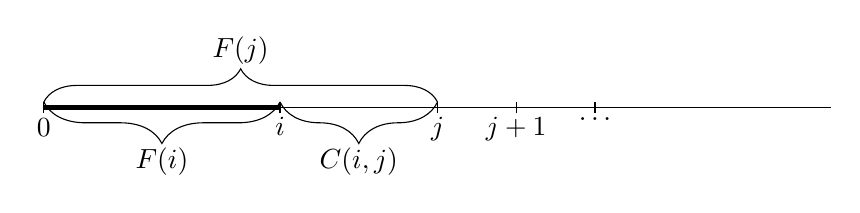
\begin{tikzpicture}
        \draw[ultra thick] (0,0)  node [below] {$0$} -- (3,0);
        \draw (3,0)  node [below] {$i$} -- (5,0);
    	\path (3,2pt) edge [draw]  ++(0,-2pt);
        \draw (5,0)  node [below] {$j$} -- (6,0);
       	\path (5,2pt) edge [draw]  ++(0,-4pt);
        \draw (6,0)  node [below] {$j+1$} -- (7,0);
        \path (6,2pt) edge [draw]  ++(0,-4pt);
        \path (7,2pt) edge [draw]  ++(0,-4pt);
        \draw (7,0)  node [below] {$\dots$} -- (10,0);
        
        \coordinate (p) at (0,3pt);
        
        \draw [decorate,decoration={brace,mirror, amplitude=15}] (0,2pt) edge [draw] +(0,-4pt) -- ++(3,0) coordinate (p) node [midway, below=(30), anchor=south] {$F(i)$};
        
        \draw [decorate,decoration={brace,mirror, amplitude=15}] (3,2pt) edge [draw] +(0,-4pt) -- ++(2,0) coordinate (p) node [midway, below=(30), anchor=south] {$C(i,j)$};
        
        \draw [decorate,decoration={brace,amplitude=12}] (0,2pt) edge [draw] +(0,-4pt) -- ++(5,0) coordinate (p) node [midway, above=(10), anchor=south] {$F(j)$};
    \end{tikzpicture}
    \caption{$F(j)$ is calculated using the best $i < j$ in terms of  $F(i) + C(i,j)$.}
    \label{dynamic_programming_1D_schema}
\end{figure}

Formally, we will start with $F(0) = 0$, and incrementally at iteration $j$, we will define $F(j) = \underset{0\leq i < j}{\min} \{ F(i) + C(i,j) + \beta \}$. We can see that the term involving $\beta$ has no influence on the value of $i$ that minimises the expression (that is $argF(j)$), the reason for the term is that we want that value stored in the container, so that future evaluations that use $F(j)$ take into account the penalization of having added a changepoint at $j$ (without that penalization term, if $C(i,i+1)$ is very small for each $i$, then the optimal solution would probably involve almost every point as changepoint).

\begin{algorithm}[H]
\caption{Optimal Partition (penalization based)}\label{optimal_partition_penalization_based}
\begin{algorithmic}[1]
\Require $C, \beta, n$ as cost function, penalization term and size of the series. 
\Ensure $F(j)$ will store the optimal value in terms of \ref{penalization_cost_function} for the prefix $[0,j)$ and $argF(j)$ will store the position where the rightmost changepoint is located when solving the problem in the $[0,j)$ prefix. 
\State $F(0) \leftarrow 0$

\State 
\rlap{\smash{$\left.\begin{array}{@{\hspace{64pt}}c@{}}\\{}\\{}\end{array}\color{gray}\right\}%
          \color{gray}\begin{tabular}{c} Initialization.\end{tabular}$}}
\State$argF(0) \leftarrow -1$
\Comment{-1 is fitting, because it is not a valid index}
\State

\For{$j \in \{1, \dots, n\}$} \Comment{$\mathcal{O}$(n) iterations}
  \State $F(j) \leftarrow \underset{i \in \{0, \dots, j-1\}}{\min} \{ F(i) + C(i,j) + \beta \}$ \Comment{$\mathcal{O}$(n)}
  \State $argF(j)\leftarrow \underset{i \in \{0, \dots, j-1\}}{\arg \min} \{ F(i) + C(i,j) + \beta \}$ \Comment{$\mathcal{O}$(n)}
\EndFor
\State \Return $F, argF$
\end{algorithmic}
\end{algorithm}

The algorithm \ref{optimal_partition_penalization_based} clearly runs in $\mathcal{O}(n^2)$, which may seem appropriate, since that is the time complexity that we had for pre-computing the values in the cost function. The problem with this approach is that we may need to run the algorithm many times for different values of $\beta$.

Once this algorithm finishes, in order to retrieve the changepoints we have to traverse the values stored in a backward fashion, starting with $n$, the changepoints will be located at $\tau_{D} = argF(n)$, $\tau_{D-1} = argF(\tau_{D}) =  argF(argF(n))$, and so on until reaching the point where the result of $argF(\dots(argF(n)\dots)$ is equal to $-1$.

Adding a reasonable hypothesis, we can derive a pruned version of \ref{optimal_partition_penalization_based}. Concretely, the hypothesis is that there exists a constant $K$ (that will play a similar role to the penalization term $\beta$, comparing with \ref{changepoint_condition}) such that for all triplets $(u, v, w)$ where $u < v < w$ the following condition holds.
\begin{equation}
    C(u, v) + C(v,w) + K \leq C(u,w)
    \label{pruning_reasonable_hypothesis_1}
\end{equation}
The idea behind the pruning is that since $F(v) = \underset{0\leq u < v}{\min} \{ F(u) + C(u,v) + \beta \}$, then since $0 \leq u < v$ it follows that 
\begin{equation}
    F(v) \leq F(u) + C(u,v) + K.
    \label{pruning_reasonable_hypothesis_2}
\end{equation} 

Now, given a certain $w > v$ we would like to prove that among all the possible locations for the rightmost changepoint when calculating the value of $F(w)$, there is no need to evaluate $u$ as a possible location, since it is $\textit{dominated}$ by the value attained at $v$. We know that $F(w) = \underset{0\leq i < w}{\min} \{ F(i) + C(i,w) + \beta \}$, hence it is enough to show that the value obtained at $v$ is smaller
\begin{align}
    F(v) + C(v, w) + K & \leq F(u) + C(u,w) + K \nonumber \iff \\
    \iff \underbrace{F(v)}_{\boxed{A}} + \underbrace{C(u,v) + C(v, w) + K}_{\boxed{B}} & \leq \underbrace{F(u) + C(u,v) + K}_{\boxed{A}} + \underbrace{C(u,w)}_{\boxed{B}}.
    \label{pruning_domination}
\end{align}

In order to obtain \ref{pruning_domination} we simply add $C(u,v)$ at both sides of the equation, and we can see that it holds because the inequality holds when we compare specific terms in the right hand side with specific terms in the left hand side. Concretely, we can see that the inequality \ref{pruning_domination} is valid because of \ref{pruning_reasonable_hypothesis_1} and \ref{pruning_reasonable_hypothesis_2}.

All these conditions allows us to prune from the search all those values that are \textit{dominated} by another, and reduce the search space where the minimum is attained at each iteration.

\begin{algorithm}[H]
\caption{Optimal Partition Pruned (penalization based, PELT)}\label{optimal_partition_penalization_based_pruned}
\begin{algorithmic}[1]
\Require $C, \beta, n$ as cost function, penalization term and size of the series. 
\Ensure $F(j)$ will store the optimal value in terms of \ref{penalization_cost_function} for the prefix $[0,j)$ and $argF(j)$ will store the position where the rightmost changepoint is located when solving the problem in the $[0,j)$ prefix. 
\State $F(0) \leftarrow 0$
\State $argF(0) \leftarrow -1$
\rlap{\smash{$\left.\begin{array}{@{}c@{}}\\{}\\{}\end{array}\color{gray}\right\}%
          \color{gray}\begin{tabular}{ccc} \\ \\ Initialization.\end{tabular}$}}
          \Comment{-1 is fitting, because it is not a valid index}
\State $\mathcal{S} \leftarrow \{0 \}$ 

\For{$j \in \{1, \dots, n\}$} \Comment{$\mathcal{O}$(n) iterations}
  \State $F(j) \leftarrow \underset{i \in \mathcal{S}}{\min} \{ F(i) + C(i,j) + \beta \}$ \Comment{$\mathcal{O}$(n)}
  \State $argF(j)\leftarrow \underset{i \in \mathcal{S}}{\arg \min} \{ F(i) + C(i,j) + \beta \}$ \Comment{$\mathcal{O}$(n)}
  \State $\mathcal{S} \leftarrow \{i \in \mathcal{S} : F(j) > F(i) + C(i,j) + K \} \cup \{j\}$ \Comment{$\mathcal{O}$(n)}
\EndFor
\State \Return $F, argF$
\end{algorithmic}
\end{algorithm}

The worst case complexity for \ref{optimal_partition_penalization_based_pruned} is $\mathcal{O}(n^2)$, and keeping at all times only the values that are not dominated would not seem have been very beneficial. In practice however, there is a significant gain with this prune, and under a special set of hypotheses and circumstances it has been reported to run in linear time \citep{killick}.


\subsection{Optimal Partition - changepoints in state}\label{changepoints_in_state}

So far we have been dependant on choosing a suitable penalization term ($\beta$). Would we be able to guess the penalization term to obtain the correct amount of changepoints by watching a visualization of the series? Probably not. On the other hand, would we be able to guess the amount of changepoints? Not necessarily, but much more likely. So despite its relation with the amount of changepoints obtained (greater penalization implies fewer changepoints), the penalization term is not something intrinsic to the problem at hand. That is why developing a solution approach that does not depend on choosing a penalization seems reasonable.

Bearing that in mind, the idea is to have a greater state in our recursion. We will still calculate the solution for each possible prefix $[0,j)$, but now we will also do it for each possible amount of changepoints. In short, we will store $F(d,j)$, where each entry will have the \textit{best possible value that we can achieve in the prefix $[0,j)$ if we choose exactly $d$ changepoints}. How do we calculate $F(d,j)$? If we assume that we know $F(d-1,i)$ for each $i < j$, then we can try all the different possibilities for the position of the rightmost changepoint when solving the prefix $[0,j)$. This would yield an $\mathcal{O}(Dn^2)$ approach, where $D$ is a bound for the amount of changepoints present (or simply our guess). If we calculate the values incrementally on $d$, then for a fixed value of $d$ we need to store $n$ values, and each one of them takes an $\mathcal{O}(n)$ search in the prefix, as we can see in algorithm \ref{optimal_partition_changepoints_in_state}.

\begin{algorithm}[H]
\caption{Optimal Partition (changepoints in state)}\label{optimal_partition_changepoints_in_state}
\begin{algorithmic}[1]
\Require $C, n, D$ as cost function, size of the series and maximum amount of changepoints in the series. 
\Ensure $F(d,j)$ stores the optimal value in terms of \ref{penalization_cost_function} (with $\beta = 0$) for the prefix $[0,j)$ using exactly $d$ changepoints, and $argF(d,j)$ stores where the optimal rightmost changepoint is located when calculating $F(d,j)$. 

\For{$j \in \{0, \dots, n\}$} 
    \State $F(0,j) \leftarrow +\infty$
    \rlap{\smash{$\left.\begin{array}{@{\hspace{10pt}}c@{}}\\{}\\{}\end{array}\color{gray}\right\}%
          \color{gray}\begin{tabular}{c}Initialization.\end{tabular}$}}
    \State $argF(0,j) \leftarrow -1$
    
\EndFor 


\For{$d \in \{1, \dots, D\}$} \Comment{$\mathcal{O}$(D) iterations}
    \State $F(d,0) \leftarrow 0$ \rlap{\smash{$\left.\begin{array}{@{\hspace{10pt}}c@{}}\end{array}\color{gray}\right\}%
          \color{gray}\begin{tabular}{c}Initialization\end{tabular}$}}
    \For{$j \in \{1, \dots, n \}$} \Comment{$\mathcal{O}$(n) iterations}
    \State $F(d,j) \leftarrow \underset{i \in \{0, \dots, j-1\}}{\min} \{ F(d-1,i) + C(i,j)\}$ \Comment{$\mathcal{O}$(n)}
  \State $argF(d,j)\leftarrow \underset{i \in \{0, \dots, j-1\}}{\arg \min} \{ F(d-1,i) + C(i,j)\}$ \Comment{$\mathcal{O}$(n)}
    \EndFor
\EndFor
\State \Return $F, argF$
\end{algorithmic}
\end{algorithm}

As we can see the only problem we have with this approach is that it takes too much time to run. One possible way to speed this is using the pruning, since under the same hypotheses, the same result follows from replacing $F(u)$ by $F(d-1,u)$ and $F(v)$ by $F(d-1, v)$ in \ref{pruning_reasonable_hypothesis_2}. By doing that we would arrive to algorithm \ref{optimal_partition_changepoints_in_state_pruned} that works relatively well in practice, but without further hypotheses, its running time can only be bounded by $\mathcal{O}(Dn^2)$ in the worst case.

\begin{algorithm}[H]
\caption{Optimal Partition Pruned (changepoints in state, PELT) }\label{optimal_partition_changepoints_in_state_pruned}
\begin{algorithmic}[1]
\Require $C, n, D$ as cost function, size of the series and maximum amount of changepoints in the series. 
\Ensure $F(d,j)$ stores the optimal value in terms of \ref{penalization_cost_function} (with $\beta = 0$) for the prefix $[0,j)$ using exactly $d$ changepoints, and $argF(d,j)$ stores where the optimal rightmost changepoint is located when calculating $F(d,j)$. 

\For{$j \in \{0, \dots, n\}$} 
    \State $F(0,j) \leftarrow +\infty$
    \rlap{\smash{$\left.\begin{array}{@{\hspace{10pt}}c@{}}\\{}\\{}\end{array}\color{gray}\right\}%
          \color{gray}\begin{tabular}{c}Initialization.\end{tabular}$}}
    \State $argF(0,j) \leftarrow -1$
    
\EndFor 


\For{$d \in \{1, \dots, D\}$} \Comment{$\mathcal{O}$(D) iterations}
    \State $F(d,0) \leftarrow 0$ 
    \State 
    \rlap{\smash{$\left.\begin{array}{@{\hspace{50pt}}c@{}}\\{}\\{}\end{array}\color{gray}\right\}%
          \color{gray}\begin{tabular}{c}Initialization.\end{tabular}$}}
    \State $\mathcal{S} \leftarrow \{ 0\}$
    \For{$j \in \{1, \dots, n\}$} \Comment{$\mathcal{O}$(n) iterations}
  \State $F(d,j) \leftarrow \underset{i \in \mathcal{S}}{\min} \{ F(d-1,i) + C(i,j) \}$ \Comment{$\mathcal{O}$(n)}
  \State $argF(j)\leftarrow \underset{i \in \mathcal{S}}{\arg \min} \{ F(d-1,i) + C(i,j) \}$ \Comment{$\mathcal{O}$(n)}
  \State $\mathcal{S} \leftarrow \{i \in \mathcal{S} : F(d,j) > F(d,i) + C(i,j) + K \} \cup \{j\}$ \Comment{$\mathcal{O}$(n)}
\EndFor
\EndFor
\State \Return $F, argF$
\end{algorithmic}
\end{algorithm}

Despite having relatively good running times in practice, we would like an algorithm that would ensure a better running time than $\mathcal{O}(Dn^2)$ in the worst case. We will see now an approach that works in the same fashion (incrementally in the number of changepoints and tries to prune the search space where the rightmost changepoint in a prefix is located), but that solves each one of the $\mathcal{O}(D)$ iterations in $\mathcal{O}\left (n\lg_2(n) \right )$, yielding a total $\mathcal{O}(Dn\lg_2(n) + P)$, where $P$ is a polynomial that captures the time taken to calculate all the pre-computations (which may now be the greatest term, depending on the approach taken for the cost function). 

There is a downside to this approach, if we want to guarantee optimality, we need to add the hypothesis that all pairs $(d,j)$ satisfy
\begin{equation}
    argF(d,j) \leq argF(d,j+1)
    \label{divide_and_conquer_optimality_hypothesis}
\end{equation}

We can simply view \ref{divide_and_conquer_optimality_hypothesis} as $argF$ being monotonically increasing in terms of $j$ for all fixed $d$. That is, if we visualize the values of $argF$ in a matrix, each row $d$ is monotonically increasing. Another way of visualizing this condition is to think of the incremental procedure for a fixed $d$, while we are adding points of the series solving the problem in the $[0,j)$ prefix, then the $[0, j+1)$ prefix, and so on, the location of the rightmost changepoint in the optimal solution does not decrease (either stays on its position or moves to the right).

If we assume for a moment that \ref{divide_and_conquer_optimality_hypothesis} holds, we can see how to solve the problem efficiently using what is known as \textit{Divide and Conquer Optimization} for Dynamic Programming \citep{laaksonen}. As we have said, the main approach will be the same, we will use the values of $F(d-1,\cdot)$ to find the values of $F(d,j)$ for each $j$. The novel idea is to keep two ranges. We will call the first range $[s,e)$ which denotes \textit{the values of $j$ where we still need to calculate the value of $F(d,j)$}. At the beginning of the iteration, this range is $[0,n)$. And we will call the second range $[A_s, A_e]$ which denotes \textit{the possible values where the rightmost changepoint might be located} (that is, it is guaranteed that the optimal choice is one element in the range). At the beginning of each iteration this range is $[0,n-1]$, and we will use inclusive ranges, because in this case we will reach something quite rare, which is that we will want to have consecutive ranges and include the extreme point in both ranges (the rightmost element in the range on the left and the leftmost element of the range on the right will be the same and present in both ranges).  

Then we proceed to calculate the value of $F(d, \left \lfloor \frac{s+e}{2}\right \rfloor)$. How do we do it? If we were to check for all $i < \left \lfloor \frac{s+e}{2} \right \rfloor$ there would be no gain, so the whole point is to search only in $\left [A_s, \min(\left \lfloor \frac{s+e}{2}\right \rfloor - 1, A_e]\right ]$, and the search step will look like \ref{divide_and_conquer_recurrence}.

\begin{equation}
    F\left (d, \left \lfloor \frac{s+e}{2}\right \rfloor \right ) = \underset{A_s \leq i < \min(\left \lfloor \frac{s+e}{2}\right \rfloor-1, A_e)}{\min} \{F(d-1, i) + C(i,j)\}
    \label{divide_and_conquer_recurrence}
\end{equation}

If we think in terms of the matrix where $F$ is stored, after the very first iteration we would have only calculated the middle point of row $d$ (that is $F(d, \left \lfloor \frac{s+e}{2} \right \rfloor)$), and we would know that such value was attained at $argF(d, \left \lfloor \frac{s+e}{2} \right \rfloor)$. How do we proceed?

In terms of the two ranges that we are maintaining, we still have to solve two subproblems. To the left, we have to calculate the values of $F(d,j)$ for $j \in \left [s, \left \lfloor \frac{s+e}{2} \right \rfloor \right )$, in order to do that, the key observation is that because of \ref{divide_and_conquer_optimality_hypothesis}, we can guarantee that the optimum will be attained somewhere on $\left [A_s, argF(d,\left \lfloor \frac{s+e}{2} \right \rfloor) \right]$. Similarly, to the right, we still have to calculate the values of $F(d,j)$ for $j \in \left [\left \lfloor \frac{s+e}{2} \right \rfloor + 1, e \right )$. Also, because of \ref{divide_and_conquer_optimality_hypothesis} we only need to make a linear search in the recurrence in the range $\left [argF(d,\left \lfloor \frac{s+e}{2} \right \rfloor), A_e \right ]$ due to $argF(d,\cdot)$ being monotonically increasing.


\begin{figure}[H]
    \label{divide_and_conquer_optimization_tree}
\begin{adjustbox}{max width=\textwidth}
\begin{forest}  
[\colorbox{red!30}{$\left [s,e \right )$} \colorbox{green!30}{$\left [A_s, A_e\right ]$}
    [{$\text{Solve }$ \colorbox{green!10}{$F\left (d, \left \lfloor \textcolor{red!100}{\frac{s+e}{2}} \right \rfloor \right)$}$ \text{ minimum attained at } argF \left (d, \left \lfloor \textcolor{red!100}{\frac{s+e}{2}} \right \rfloor \right )$}
        [\colorbox{red!30}{$\left [s,\frac{s+e}{2} \right)$}   \colorbox{green!30}{$\left [A_s, argF \left (d, \left \lfloor \frac{s+e}{2} \right \rfloor \right ) \right ]$}
            [{$\text{Solve }$ \colorbox{green!10}{$F\left (d, \left \lfloor \textcolor{red!100}{\frac{3s+e}{4}} \right \rfloor \right)$} $\text{ at } argF \left (d, \left \lfloor \textcolor{red!100}{\frac{3s+e}{4}} \right \rfloor \right )$}
                [\colorbox{red!30}{$\dots$}\colorbox{green!30}{$\dots$}]
                [\colorbox{red!30}{$\dots$}\colorbox{green!30}{$\dots$}]
            ]
        ]
        [\colorbox{red!30}{$\left [\frac{s+e}{2}+1, e \right)$} \colorbox{green!30}{$\left [argF \left (d, \left \lfloor \frac{s+e}{2} \right \rfloor \right ), A_e \right ]$}
            [{$\text{Solve }$ \colorbox{green!10}{$F\left (d, \left \lfloor \textcolor{red!100}{\frac{s+3e}{4}} \right \rfloor \right)$}$ \text{ at } argF \left (d, \left \lfloor \textcolor{red!100}{\frac{s+3e}{4}} \right \rfloor \right )$}
                [\colorbox{red!30}{$\dots$}\colorbox{green!30}{$\dots$}]
                [\colorbox{red!30}{$\dots$}\colorbox{green!30}{$\dots$}]
            ]
        ]
    ]
]
\end{forest}
\end{adjustbox}
\caption{Tree representation of the recursive calls using Divide \& Conquer Optimization technique.}
\end{figure}



If we visualize this recursion steps in the form of a tree like in \ref{divide_and_conquer_optimization_tree}, we can see that its depth is $\mathcal{O}(\lg_2(n))$, since the length of the first ranges is halved at each level. However, at each level, we iterate over the second range of each node to search for the optimum value (like we do in \ref{divide_and_conquer_recurrence}), and the union of these ranges makes up all $[0,n-1]$ almost without intersection (the extreme points between consecutive ranges as only exception). The important remark is that if we sum all the lengths it is bounded by $2n$ which makes the amortized complexity of the whole level to be  $\mathcal{O}(n)$. So, in total, we are doing $\mathcal{O}(n)$ operations per level, and since there are only $\mathcal{O}(\lg_2(n))$ levels, we can now solve for each value of $d$ in $\mathcal{O}(n\lg_2(n))$, which gives us a total complexity of $\mathcal{O}(Dn\lg_2(n))$ wihtout taking into account the pre-computations.


\begin{algorithm}[H]
\caption{Calculate in range (changepoints in state, D\&C optimization) }\label{calculate_range_divide_and_conquer}
\begin{algorithmic}[1]
\Require $C, s, e, A_s, A_e$ and $d$ as cost function, start of first range, end of first range, start of second range, end of second range and the amount of changepoints of the subproblem.
\Ensure $F(d,j)$ stores the heuristic value in terms of \ref{penalization_cost_function} (with $\beta = 0$) for the prefix $[0,j)$ using exactly $d$ changepoints, and $argF(d,j)$ stores where the optimal rightmost changepoint is located when calculating $F(d,j)$. 
\State $m \leftarrow \left \lfloor \frac{s+e}{2} \right \rfloor$
\State $F(d,m)\leftarrow \underset{A_s \leq i \leq \min(m-1, A_e)}{\min} \left \{F(d-1,i) + C(i,j) \right \}$
\State $argF(d,m) \leftarrow \underset{A_s \leq i \leq \min(m-1, A_e)}{\arg \min} \left \{F(d-1,i) + C(i,j) \right \}$
\If{$m > s$}
    \State Use algorithm \ref{calculate_range_divide_and_conquer} recursively in $[s, m)$, searching in $[A_s, argF(d,m)]$.
\EndIf
\If{$m+1 < e$}
    \State Use algorithm \ref{calculate_range_divide_and_conquer} recursively in $[m+1, e)$, searching in $[argF(d,m), e]$.
\EndIf

\end{algorithmic}
\end{algorithm}


\begin{algorithm}[H]
\caption{Heuristic partition (changepoints in state, D\&C optimization) }\label{heuristic_partition_changepoints_in_state_divide_and_conquer}
\begin{algorithmic}[1]
\Require $C, n, D$ as cost function, size of the series and maximum amount of changepoints in the series. 
\Ensure $F(d,j)$ stores the heuristic value in terms of \ref{penalization_cost_function} (with $\beta = 0$) for the prefix $[0,j)$ using exactly $d$ changepoints, and $argF(d,j)$ stores where the optimal rightmost changepoint is located when calculating $F(d,j)$. 

\For{$j \in \{0, \dots, n\}$} 
    \State $F(0,j) \leftarrow +\infty$
    \rlap{\smash{$\left.\begin{array}{@{\hspace{10pt}}c@{}}\\{}\\{}\end{array}\color{gray}\right\}%
          \color{gray}\begin{tabular}{c}Initialization.\end{tabular}$}}
    \State $argF(0,j) \leftarrow -1$
    
\EndFor 


\For{$d \in \{1, \dots, D\}$} \Comment{$\mathcal{O}$(D) iterations}
    \State $F(d,0) \leftarrow 0$ \rlap{\smash{$\left.\begin{array}{@{\hspace{10pt}}c@{}}\end{array}\color{gray}\right\}%
          \color{gray}\begin{tabular}{c}Initialization.\end{tabular}$}}
        \State Use algorithm \ref{calculate_range_divide_and_conquer} in $[0, n)$, searching in $[0, n-1]$ at level $d$.
\EndFor
\State \Return $F, argF$
\end{algorithmic}
\end{algorithm}




The counterpoint of the strategy described in \ref{heuristic_partition_changepoints_in_state_divide_and_conquer} is that depending on the time series values and the cost function chosen, the hypothesis \ref{divide_and_conquer_optimality_hypothesis} might not hold, ruining the proof of its optimality. On the other hand, the time complexity analysis remains unaltered, if we define the ranges in the same way, we will achieve $\mathcal{O}(Dn\lg_2(n))$ complexity, since each consecutive ranges still overlap at most at the extreme points (which allows us to bound each level of the tree in $\mathcal{O}(n)$), and the depth of the tree is still at most $\mathcal{O}(\lg_2(n))$. So this technique can still be used, but only as a heuristic that works fast to solve the problem without proven optimality. We will see in future sections that it still shows very good results in terms of its quality, while achieving a significant improvement in terms of running time.


\section{Input generation}\label{input}

In order to test the algorithms that we implemented we need test cases. We created two types of test cases. The first one involves random sampled generated data from different distributions. The second one involves the real measurement of the beats per minute among a two month period. Aside from the time series $y$, we will also discuss how to generate sensible values for the penalization term ($\beta$) and a guess about the amount of changepoints ($D$).

\subsection{Randomly generated data}

We created 15 test cases for each distribution. Case number $i$ has $i\cdot 1000$ values. Once the length $n$ of the series was set, we selected $D$ the amount of changepoints in that series to be a random number of magnitude $\mathcal{O}(\ln(n))$ (concretely, a random integer between $\frac{1}{2}\ln(n)$ and $2\ln(n)$). Also, for each $i$ we sampled:
\begin{itemize}
    \item $\mu_{low}$ a uniform random integer between $-15$ and $0$.
    \item $\mu_{high}$ a uniform random integer between $0$ and $15$.
    \item $\sigma_{low} = 1$ 
    \item $\sigma_{high}$ a uniform random integer between $2$ and $8$.
    \item $\lambda_{low} = 1$ 
    \item $\lambda_{high}$ a uniform random integer between $2$ and $10$.
    \item $\mu$ a uniform random integer between $\mu_{low}$ and $\mu_{high}$.
    \item $\sigma$ a uniform random integer between $\sigma_{low}$ and $\sigma_{high}$.
\end{itemize}

Once we have these values, we generate the locations where we will put the changepoints by sampling $D$ numbers without replacement from the range $\{1, \dots, n-1\}$. Then, knowing the locations of the changepoints, for each distribution we created a time series of $n$ values that changes an aspect of the underlying distribution at each of the sampled changepoints.



The important aspect of creating the cases is that we know the location of the changepoints, so we can test whether our algorithms are able to detect them or not in each scenario. For the case of a Gaussian distribution, between each changepoint in one set of test cases the mean was changed to a new uniformly real value between $\mu_{low}$ and $\mu_{high}$. In other set of Gaussian test cases, the variance was changed to a new uniformly real value between $\sigma_{low}$ and $\sigma_{high}$. For the exponential distribution a new uniformly real value between $\lambda_{low}$ and $\lambda_{high}$ was chosen at each changepoint. Lastly, another set of data was generated where each value was not independent from the others. Concretely, each value was a convex combination of the three previous values, plus a Gaussian value that changed its mean at each changepoint.

\subsection{Real data}

We also added to the data set some real instances using measurements of the beats per minute among a two month period. Since two months involves a lot of values, we took only random contiguous segments of at most 15000 values (about 10 days). The idea is that in this signal we should be able to detect sleep cycles since they would result in a decrease in the average number of beats per minute. We could also be able to find a relatively long physical activity (running for example), but they should not appear as often in the data.

\subsection{Selection of penalization and number of changepoints}

\textcolor{red}{Hablar no solo de c\'omo se generan los casos, sino tambi\'en de cómo se utilizan los greedys/heur\'isticas que funcionan r\'apido para elegir un número razonable de cota de changepoints y penalizaci\'on}

\section{Results}\label{results}

\textcolor{red}{Pegar tablitas con distintas muestras, los valores de la funci\'on objetivo, el tiempo que tard\'o en cada uno, falsos positivos, etc\'etera}

Basicamente se corrre el greedy primero y despues con los changepoints se divide a la señal en secciones (cada punto de la señal pertence a la sección definida por el par de changepoints consecutivos entre los que está comprendido). Entre otra cosas, se evalua con la funcion de costos para cada punto.Para cada punto de la señal, se calcula un numero (silhouette), que intenta aproximar cuan bien asignado esta en su seccion el coso. 





\textcolor{red}{Releer}


\bibliography{sn-bibliography}

\end{document}
